% AgentLedger -- Phase 2 paper template (IEEEtran, conference mode)
% Upload this whole `paper/` folder to Overleaf (or compile locally with
% pdflatex + bibtex). Structure, section headers, and the real data
% tables/figures are filled in; the analysis prose in each section is marked
% [[WRITE THIS: ...]] for you and Areej to write in your own words -- do not
% submit this file with those markers still in it, and do not have an AI
% write the prose that replaces them (the brief requires original writing,
% checked by Turnitin's AI report).
%
% TODO before submitting:
%  - Fill in author names/roll numbers/emails below.
%  - Replace every [[WRITE THIS: ...]] block with your own prose.
%  - Fill in Gap 2's rows/sections once Areej's work lands.
%  - Get the page count to 8-10 (currently a skeleton, will grow as you write).
%  - Verify every reference in references.bib and add more to reach 25-30.

\documentclass[conference]{IEEEtran}
\usepackage{cite}
\usepackage{graphicx}
\usepackage{booktabs}
\usepackage{amsmath}
\usepackage{hyperref}

\begin{document}

\title{AgentLedger: Evidence-Bound, Tamper-Evident, Control-Mapped Auditing of Agent Logs}

\author{
\IEEEauthorblockN{Armish Tauqir}
\IEEEauthorblockA{Roll No. 23i-0786 \\ National University of Computer and Emerging Sciences \\ [[TODO: email]]}
\and
\IEEEauthorblockN{Areej Fahim}
\IEEEauthorblockA{Roll No. 23i-0504 \\ National University of Computer and Emerging Sciences \\ [[TODO: email]]}
}

\maketitle

% ============================================================
\begin{abstract}
[[WRITE THIS, 150-250 words: state the problem (agent logs aren't audit
evidence), your approach (three gap-specific components: evidence-bound
Auditor+Verifier for Gap 1, a hash-chained Integrity Ledger with provenance
for Gap 2, a control-mapped Policy Checker for Gap 3), your main
quantitative result (lead with the unsupported-claim rate finding: 0\% with
the Verifier vs. 56\% without it on real Who\&When data -- this is your
strongest, cleanest number), and your contribution in one sentence. Write
this section LAST, after the Results section is final, so the numbers you
quote here match exactly.]]
\end{abstract}

% ============================================================
\section{Introduction}
[[WRITE THIS: motivate the problem (agent logs today are unstructured,
unverifiable transcripts -- not evidence), state the three research gaps
from Phase 1 (Gap 1: findings without evidence; Gap 2: no tamper-evidence
on agent run logs; Gap 3: safety checks that don't map to named regulatory
controls), your research questions (see Problem Formulation below for the
exact H1/H2/H3 wording to reuse), and a short bullet list of contributions,
e.g.:
\begin{itemize}
  \item An Auditor--Retriever--Verifier pipeline that cites specific log
    records for every finding and rejects claims the cited records don't
    support.
  \item A SHA-256 hash-chained Integrity Ledger [[Areej: your provenance
    graph detail here]].
  \item A control catalogue (ISO/IEC 42001 + NIST AI RMF) and Policy
    Checker mapping trajectories to named compliance controls.
  \item An empirical comparison against the base paper (Who\&When
    \cite{zhang2025whowhen}) on real data, including an ablation isolating
    exactly what the Verifier buys you.
\end{itemize}
]]

% ============================================================
\section{Related Work}
[[WRITE THIS: synthesize the Phase 1 literature review (see
\texttt{doc/Agentic Phase 1 (fixed).docx}, section A3) rather than
re-listing it -- group by theme (failure attribution
\cite{zhang2025whowhen,cemri2025mast,zhang2026agentracer}, LLM-as-judge
safety evaluation \cite{luo2025agentauditor,zheng2023llmjudge}, guardrail/
policy agents \cite{chen2025shieldagent,wang2026agentspec,xiang2025guardagent},
provenance and tamper-evidence \cite{souza2025provagent,li2026auditablellm},
compliance auditing \cite{zheng2026audagent,ameur2025eurocomply,macbench2026})
and explicitly position AgentLedger against each group: what they do that we
build on, and what gap in each remains that our system addresses. End by
restating, in one sentence per gap, how AgentLedger differs from the closest
prior work.]]

% ============================================================
\section{Problem Formulation}
Building on Phase 1, we define three gap-specific hypotheses, tested
empirically in Section~\ref{sec:results}:

\begin{itemize}
  \item \textbf{H1 (Gap 1).} Requiring an Auditor to cite specific log
  records for its claim, and a Verifier to reject claims the cited records
  don't support, reduces the rate of \emph{unsupported claims} (claims
  marked trustworthy that are actually wrong) relative to citing without
  verification.
  \item \textbf{H2 (Gap 2).} [[Areej: restate your tamper-detection
  hypothesis and target numbers from Phase 1 here once that experiment is
  run.]]
  \item \textbf{H3 (Gap 3).} Mapping a ledgered trajectory to a named
  control catalogue (ISO/IEC 42001, NIST AI RMF) via explicit
  trigger/predicate rules detects planted compliance violations with high
  precision and recall, something no baseline in our comparison set
  measures at all.
\end{itemize}

[[WRITE THIS: 1-2 paragraphs giving the precise task definition -- input
(a RunLog: a normalised sequence of Events, each with an agent, step index,
content, and tool calls -- see \texttt{src/agentledger/schema.py}), output
(an \texttt{AuditFinding}: agent, step, control\_id, passed, cited record
ids, verified flag -- see \texttt{src/agentledger/orchestrator.py}), and the
two concrete tasks evaluated: failure attribution (agent + step, scored
against Who\&When's ground truth) and control-compliance checking (pass/
fail per control, scored against the injected-violation suite's planted
ground truth).]]

% ============================================================
\section{Proposed System / Methodology}
Figure~\ref{fig:arch} shows the architecture. \texttt{src/agentledger/orchestrator.py}'s
\texttt{run\_system()} is the single entry point: a Retriever shortlists
candidate log records, an Auditor proposes an agent/step claim citing
specific record ids from that shortlist, a Verifier re-reads only the cited
records and either accepts or rejects the claim (with one revision pass on
rejection), and a Policy Checker runs every implemented control predicate
over the ledgered trajectory. The Integrity Ledger's chain-verification
result gates every finding: a broken chain forces every finding to
\texttt{verified=False} regardless of what the Verifier concluded.

\begin{figure}[t]
  \centering
  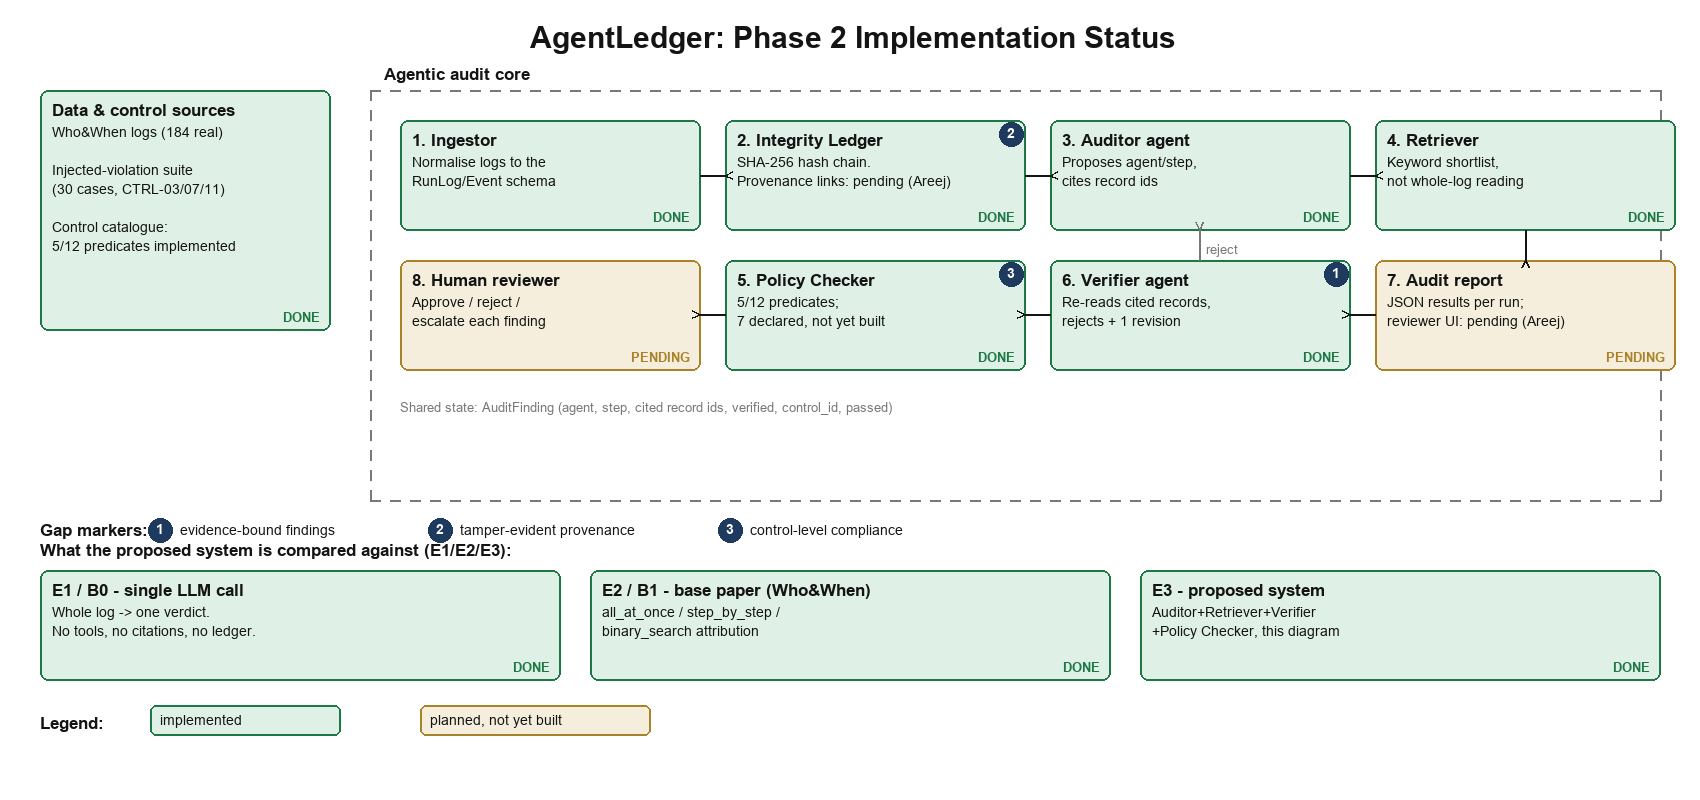
\includegraphics[width=\columnwidth]{figure2_phase2_status.png}
  \caption{AgentLedger architecture and Phase 2 implementation status. Gap
  markers: 1 = evidence-bound findings (Auditor/Verifier), 2 = tamper-evident
  provenance (Integrity Ledger), 3 = control-level compliance (Policy
  Checker).}
  \label{fig:arch}
\end{figure}

\subsection{Gap 1: Auditor, Retriever, Verifier}
[[WRITE THIS: describe the Retriever's candidate-shortlisting approach
(error-keyword search + tail window, \texttt{src/agentledger/agents/retriever.py}),
the Auditor's prompt/output contract (cites record ids, JSON-structured,
\texttt{agents/auditor.py}), and the Verifier's accept/reject/revise loop
(\texttt{agents/verifier.py}). Justify why this is agentic (ties to Phase
1's B5 agentic-justification argument: retrieval instead of whole-log
reading, a multi-step plan-act-observe loop, tool calls, revision on
rejection) rather than a single prompt.]]

\subsection{Gap 2: Integrity Ledger}
[[Areej: WRITE THIS -- describe the SHA-256 hash chain
(\texttt{src/agentledger/ledger.py}) and your provenance-graph extension.]]

\subsection{Gap 3: Control Catalogue and Policy Checker}
[[WRITE THIS: describe the control catalogue (12 controls declared, 5
implemented: CTRL-01 complete ledgered record-keeping, CTRL-02 tool calls
logged, CTRL-03 human oversight before high-risk tool calls, CTRL-07
corrective action after an error step, CTRL-11 no sensitive data in tool
arguments -- \texttt{src/agentledger/controls.py}) and the Policy Checker
that runs them over a ledgered trajectory (\texttt{agents/policy\_checker.py}).
Be explicit that 7 controls remain declared-but-unimplemented and are
skipped, not silently passed.]]

% ============================================================
\section{Experimental Setup}
\textbf{Data.} The real Who\&When benchmark \cite{zhang2025whowhen} (184
annotated multi-agent failure logs: 58 Hand-Crafted + 126
Algorithm-Generated), loaded via \texttt{load\_whowhen\_release\_full}. All
results in this paper use a fixed [[N -- state 20 or 40, whichever sample
you finalize]]-log subset (10/20 Hand-Crafted + 10/20 Algorithm-Generated,
first-by-file-order -- not hand-picked) [[WRITE THIS: state plainly that the
full 184-log benchmark was not run due to the free-tier evaluation
timeline, and that this is a directional, not final, result -- honesty here
is explicitly rewarded by the grading rubric]]. The Gap 3 injected-violation
suite (\texttt{data/injected\_violations/}, 30 synthetic cases, 10 each for
CTRL-03/07/11) provides planted ground truth where Who\&When has none.

\textbf{Models.} All real-data runs use Groq's free-tier API. Because each
model is capped at roughly 200{,}000 tokens/day on the free tier,
\texttt{GroqProvider} (\texttt{src/agentledger/providers.py}) falls through
a chain of models (\texttt{qwen/qwen3.8-27b} $\rightarrow$
\texttt{openai/gpt-oss-120b} $\rightarrow$ \texttt{openai/gpt-oss-20b}
$\rightarrow$ \texttt{openai/gpt-oss-safeguard-20b} $\rightarrow$
\texttt{allam-2-7b}) whenever the current model's daily quota is hit; each
result file's \texttt{provider\_stats.model\_switches} records which models
a given run actually used. [[WRITE THIS: 1-2 sentences stating that model
identity therefore varies run-to-run on the free tier, which is itself a
reliability finding discussed in Section~\ref{sec:ablation}, and is a clear
threat to validity discussed in Section~\ref{sec:limitations}.]]

\textbf{Baselines.} E1 is baseline B0 (whole log, one prompt, bare verdict).
E2 is the base paper's own \texttt{all\_at\_once} attribution method,
re-implemented against our schema (\texttt{src/agentledger/baselines/}).
[[WRITE THIS: state plainly that \texttt{step\_by\_step} and
\texttt{binary\_search} were only run on the small synthetic sample, not
the real subset, due to their much higher per-run call count under the
free-tier time budget -- see \texttt{results/baseline\_b1\_results.json}
for those synthetic-sample numbers if you want to mention them.]]

% ============================================================
\section{Evaluation Methodology}
\textbf{Metrics.} Agent-level and step-level accuracy (exact match against
Who\&When's \texttt{responsible\_agent}/\texttt{decisive\_step}); grounded-
correct count and \emph{unsupported-claim rate} (share of findings marked
\texttt{verified=True} that are actually wrong -- the key new Gap 1 metric,
computed in \texttt{results/gap1\_ablation\_summary.json}); control-level
precision/recall/F1 against the injected-violation suite's planted ground
truth (\texttt{eval/run\_policy\_eval.py}); call count, latency, and prompt/
completion character volume per run (\texttt{LLMProvider.stats()}).

\textbf{Base-paper comparison.} E2's numbers in Table~\ref{tab:gap1gap3} are
reproduced by us on the same 20-log real subset and the same metrics as
E1/E3, not taken from the original paper's reported 53.5\%/14.2\% (which
were measured on the full 127/184-system benchmark with a different model).

% ============================================================
\section{Results}
\label{sec:results}

\begin{table}[t]
\centering
\caption{Gap-resolution table (n=20 real Who\&When logs). See
\texttt{results/gap\_resolution\_table\_gap1\_gap3.md} for reproduction
commands.}
\label{tab:gap1gap3}
\small
\begin{tabular}{@{}lllc@{}}
\toprule
Gap & Metric & Base paper (E2) & Ours (E3) \\
\midrule
1 & Agent acc. & 40.0\% & 40.0\% \\
1 & Step acc. & 25.0\% & 20.0\% \\
1 & Unsupported-claim rate & n/a & \textbf{0.0\%} \\
2 & Tamper detection & --- & [[Areej]] \\
3 & Control F1 (5 predicates) & n/a & 1.00 \\
\bottomrule
\end{tabular}
\end{table}

\begin{table}[t]
\centering
\caption{Gap 1 ablation: Verifier on vs.\ off (n=20).}
\label{tab:ablation}
\small
\begin{tabular}{@{}lcc@{}}
\toprule
 & Verifier ON & Verifier OFF \\
\midrule
Agent accuracy       & 40.0\% & 35.0\% \\
Step accuracy        & 20.0\% & 5.0\%  \\
Verified rate        & 5.0\%  & 80.0\% \\
Unsupported-claim rate & \textbf{0.0\%} & 56.3\% \\
\bottomrule
\end{tabular}
\end{table}

[[WRITE THIS: walk through Table~\ref{tab:gap1gap3} and
Table~\ref{tab:ablation} gap by gap. For Gap 1, be honest that raw accuracy
is roughly on par with the reproduced base-paper method at this sample
size -- the real result is the unsupported-claim rate. For Gap 3, state
the F1=1.00 result and its caveat (deterministic rules scored on the
patterns they were built to detect -- see
\texttt{results/e5\_ablation\_gap3.md}). Pull 2-3 concrete numbers from
\texttt{results/failure\_analysis\_gap1.md} to illustrate. [[Areej: add
Gap 2's row and paragraph once your tamper-test results land.]]]]

% ============================================================
\section{Ablation \& Comparative Analysis}
\label{sec:ablation}
[[WRITE THIS: reference Table~\ref{tab:ablation} again from the efficiency
angle -- see \texttt{results/e6\_efficiency.md} for the full cost/latency
breakdown (E3 makes $\sim$3.35 LLM calls/run vs. 1.0 for either baseline,
at a similar average per-call latency). Discuss the free-tier model-fallback
mechanism itself as a reliability result: it recovered automatically from a
daily-quota exhaustion mid-run with zero manual intervention in the E1/E2
reruns (see \texttt{provider\_stats.model\_switches}), whereas pre-fix runs
(\texttt{results/system\_results\_noverifier.json}) show 4/20 runs failing
outright. [[Areej: add your Gap-3-component-removed-vs-present cost
comparison once relevant, or reference
\texttt{results/e5\_ablation\_gap3.md}'s explanation of why that specific
ablation is measured on the injected-violation suite instead.]]]]

% ============================================================
\section{Failure Analysis}
[[WRITE THIS from \texttt{results/failure\_analysis\_gap1.md}, which
already has: a 5-category breakdown with frequencies (40\% incorrect
abstention, 20\% correct-agent-wrong-step, 20\% fully correct, 15\%
orchestrator-attribution-bias, 5\% infra error), two success cases
(\texttt{e142056d...}, \texttt{42d4198c...}) and two failure cases
(\texttt{d1af70ea...}, \texttt{0a65cb96...}) with real trajectory excerpts
and a stated likely cause for each. Turn that file's bullet points into
prose here -- don't just copy it verbatim, since it was drafted as your
working notes, not paper text.]]

% ============================================================
\section{Limitations \& Threats to Validity}
\label{sec:limitations}
[[WRITE THIS. Candidates already identified in this session's work (expand
in your own words, don't just list):
\begin{itemize}
  \item Small sample (n=20, not the full 184-log benchmark) -- directional,
    not final, numbers.
  \item Free-tier model identity varies run to run (fallback chain), so
    results aren't attributable to one fixed model.
  \item The Verifier's precision/recall trade-off is untuned -- its
    acceptance bar may be stricter than necessary (see Failure Analysis).
  \item Gap 3's F1=1.00 is on deterministic rules scored against the exact
    patterns they detect, not validated against real or human-labelled
    violations (a limitation Phase 1's own supervisor feedback flagged).
  \item [[Areej: your Gap 2 threats -- e.g. synthetic vs. real tamper
    patterns, provenance graph completeness.]]
\end{itemize}
]]

% ============================================================
\section{Conclusion}
[[WRITE THIS: 1 paragraph restating the main finding (citation + verification
measurably reduces unsupported claims, at a real coverage cost) and a short,
concrete future-work list: run the full 184-log benchmark; tune the
Verifier's acceptance threshold and re-measure the precision/recall
trade-off; validate Gap 3's predicates against real/human-labelled
violations; [[Areej: add Gap 2 future work]].]]

% ============================================================
\bibliographystyle{IEEEtran}
\bibliography{references}

\end{document}
